\documentclass[a4paper,12pt]{article}

% 导言区
\usepackage{titlesec}
\usepackage{lipsum} % 示例用,可以删除
\usepackage{geometry}
\usepackage{setspace}
\usepackage{amsmath} % 用于数学公式
\usepackage{graphicx} % 用于插入图片
\usepackage{float}
\usepackage{lipsum} % 用于生成虚拟文本
\usepackage{ctex} % 导入 ctex 包以支持中文
\usepackage{titlesec} % 导入 titlesec 包以定制标题样式
\usepackage{fontspec} % 用于设置中文字体
\usepackage{amsfonts}
\usepackage{amsmath} % 提供 \text 和 \tanh 命令
\usepackage{bm}      % 提供 \bm 命令用于粗体
% 目录设置
\usepackage[nottoc,notlot,notlof]{tocbibind}
\usepackage{enumitem}
% 页面设置
\geometry{margin=1in}

% 标题设置
\titleformat{\section}{\normalfont\Large\bfseries}{\thesection}{1em}{}
\titleformat{\subsection}{\normalfont\large\bfseries}{\thesubsection}{1em}{}
\titleformat{\subsubsection}{\normalfont\normalsize\bfseries}{\thesubsubsection}{1em}{}

% 行间距设置
\onehalfspacing

% 文档信息
\title{商业模式评估}
\author{需求不寄小分队}
\date{\today}

\begin{document}

    \maketitle

% 添加目录
    \tableofcontents


    \subsection{团队成员}
    211250124 程智镝

    211250122 刘辉

    211250159 陈凌

    211250158 李忠信
    \subsection{度量数值}

    \section{文档简介}
    

    \section{商业模式环境}
    \subsection{市场影响力}
    \subsubsection{市场影响力}
    \textbf{子问题1:影响客户环境的关键问题有哪些?}
    
    如何体现:哪些关键问题正在影响会议软件的市场?
    
    回答:延迟与画⾯清晰度是⼀⼤关键。优质的云服务商提供的强⼤的云服务平台与快速访问。提供更多可配置和可扩展的选项以满足不同企业的需求。提供灵活的定价计划,并确保性价比是维持市场份额的重要手段。
    
    \textbf{子问题2:哪些改变正在发生?}

    如何体现:当今的会议软件正在经历怎样的变化?

    回答:在后疫情时代,远程会议软件依然有着蓬勃的发展力。例如新闻1中提到,腾讯会议在上线2个⽉后,⽇活跃度已经突破1000万。会议软件需要注重提供支持远程协作和沟通的功能,而不再仅仅是单独的视讯与⾯对⾯交流,新闻2就提及,如何在疫情之后仍然留住这些客户,还需要根据⽤户反馈进⾏实时的调整与更新。

    \textit{调研新闻 1——⾃上线2个⽉⽇活破千万后,腾讯会议继续扩⼤着⾃⼰的影响⼒。在上线245天后,成为中国最多⼈使⽤的视频会议产品,并多次登顶APPSTORE中国区免费榜。}
    
    \rightline{\textit{——腾讯⽹:云会议市场峰回路转,远程办公迎来“腾讯时刻”?}}

    \textit{调研新闻 2——⾏业需要根据⽤户反馈的问题进⼀步做出相关调整,⽐如利⽤⼿机和电脑等硬件来开视频会议,相对还有⼀些阻碍,相关的产品或服务会有⼀个逐渐演化、完善的过程。}
    
    \rightline{\textit{———中国经营报:远程视频会议⽕爆,前景价值⼏何?}}

    
    \textbf{子问题3:市场将走向何处?}

    如何体现:对于现今的视频会议软件,未来的发展趋势是什么?

    回答:会议软件的盈利模式来⾃于客户的消费与会员制度,最需要确保的客户群是⼤公司与⼤企业的使⽤率。对许多企业来说,使⽤线上会议进⾏开会是转型的趋势。未来的视讯会议软件需要向更多元的⽅向去发展。如同新闻3所说,腾讯会议正因不断迭代的功能,才能不断吸引新的客户群体。

    \textit{调研新闻 3——腾讯会议在技术和⽤户体验上持续改进,通过最可靠的安全策略,快速迭代完善的产品功能,为更多企业的远程办公保驾护航。}

    \rightline{\textit{——腾讯⽹:⼀⽂告诉你,腾讯会议为何能成为政务企业的⾸选}}
    
    \subsubsection{市场分类}
    \textbf{子问题1:哪些是最重要的客户群体?}

    如何体现:在商业模式画布中的客户细分中,哪⼀部分客户最重要?

    回答:在客户群体⾥⾯,能提供⼤量资源与商业利益的企业必然是⾸先服务的对象。从新闻4中得知,腾讯会议总是⾯向企业服务,为企业打造最优质的办公环境与线上的会议环境。腾讯会议也因为优秀的保密算法与强⼤的云服务平台,在新闻5⾥⾯能够吸引超过1亿⼈的⽤户群体,⽽且最⾼能⽀持2000⼈在线,同时发布了腾讯会议企业版来吸引企业用户使用。

    \textit{调研新闻 4——腾讯会议已有超过1亿注册⽤户,企业微信⽇活跃账户数同⽐增⻓超过100\%。}

    \rightline{\textit{——中国新闻⽹:腾讯Q3财报:腾讯会议⽤户数破亿,云业务加速⽴标杆}}

    \textit{调研新闻 5——作为中国⽬前最多⼈使⽤的专业视频会议产品,腾讯会议已深度服务于政务、⾦融、教育、医疗等⾏业和中⼩企业在线办公,为企业级⽤户打造专属会议能⼒,最⾼⽀持2000⼈同时在线。腾讯发布腾讯会议企业版本,增强了⽹络研讨会,同声传译及连接企业原有会议室系统等功能。}

    \rightline{\textit{————中国青年⽹:Q3腾讯会议⽤户过亿 ⾦科及企业服务板块增⻓24\%}}
    
    \textbf{子问题2:哪个群体的增长潜力最大?}

    如何体现:在商业模式画布中的客户细分中,那⼀部分的客户是可积极发展商业化的⽬标群体?

    回答:最具商业潜⼒的群体是⾼校师⽣。许多⾼校发现了线上授课的诸多好处,新闻中就提到,数字化教学低成本且⾼效,可以进⾏跨区域的协作,是⼀个待开发的潜⼒客户群体。

    \textit{随着IT技术的逐步完善,我国的信息化教育也进⼊第⼆阶段,其中最典型的配合就是⾼清视频会议系统软件应⽤远程教育了,它完美的契合数字化教学的应⽤,其中就包含在线流媒体教育、远程观摩评价、远程互动教育、远程会议与培训、跨区域协作等。}

    \rightline{\textit{——腾讯⽹:⾼清视频会议系统软件助⼒教育⾏业应⽤}}

    \textbf{子问题3:哪些边缘群体值得留意?}

    如何体现:在商业模式画布中的客户细分中,那⼀部分的客户是占比较小但值得发展的⽬标群体?

    回答:国际用户可能是一个边缘群体,特别是那些在不同时区工作的组织和专业人士。
    在一些新兴市场,尤其是亚洲和非洲等地区,在支持本地语言和文化的情况下,腾讯会议可能找到增长机会。
    \subsubsection{需求与诉求}
    \textbf{子问题1:客户需要什么?}

    如何体现:客户想通过会议软件解决什么问题?

    回答:⾼校师⽣可以⽤它来进⾏远程教学、企业可以进⾏保密的线上会议、跨国⼤企业可以进⾏不断联且低延迟的通讯会议。
    
    \textbf{子问题2:客户真正想要搞定什么?}

    如何体现:客户使⽤我们的产品时最基本的需求是什么?

    回答:客户使⽤远程会议软件的最根本⽬的就是快捷与⾼效。

    \textbf{子问题3:哪些需求在增加?哪些在减少?}

    如何体现:在⼦问题1中的需求,哪⼀个需求时呈现增⻓的趋势?哪些需求其实对⽤户⽽⾔会逐渐变得不再重要?

    回答:商业中的跨国会议业务会议需求正在不断的增加。在产业链上⾯,跨国间的沟通就显得格外重要。当然,多语⾔的⽀持也是必须的。
    而对于减少的需求,⾃从复学之后,⾼校的需求正在急剧下滑。因为⼤部分的⾼校师⽣已经回到校园进⾏⾯对⾯的授课,软件必须积极进⾏转型,将产品在教师⽤户⼼中的定位从不得不⽤该产品上课,转为想使⽤该产品上课,才能留住教育群体。
    
    \subsubsection{切换成本}
    \textbf{子问题1:哪些东西将客户捆绑在一家供应商和它的服务上?}

    如何体现:有哪些服务是腾讯会议可以提供给客户⽽其他公司提供不了的?

    回答:腾讯会议作为腾讯生态系统的一部分,更容易与其他腾讯产品和服务进行集成,为用户提供更为一体化的工作体验。
    提供便捷的云端录制和存储功能,用户可以方便地保存和分享会议录音和录像。
    同时,腾讯会议具备高质量的虚拟背景和美颜功能。腾讯会议在企业版中提供一系列个性化定制选项,以及适用于企业级管理的功能。

    \textbf{子问题2:哪些切换成本阻止客户转投竞争对手?}

    如何体现:⽤户如果不使⽤我们的产品,⽽去使⽤其他的社交软件或者视频软件 ,他会失去什么?

    回答:腾讯会议具有专业的会议功能,使用其他社交软件或视频软件可能无法获得同样的专业会议体验。腾讯会议通常提供企业级的安全性和隐私保护措施,适用于敏感业务和机密信息的在线沟通。腾讯会议可能更好地集成腾讯云、腾讯文档等服务,提供更为无缝的协作体验。


    \textbf{子问题3:客户容易找到并采购类似的服务吗?}

    如何体现:现在市场上有和腾讯会议提供相似的服务的软件吗?

    回答:目前中国市场中视频软件数量较少,但是在国外有很多类似软件例如在全球范围内广泛使用,例如Zoom、Microsoft Teams、Skype。

    \textbf{子问题4:品牌有多重要?}

    如何体现:竞争市场上有巨头式的知名软件吗?腾讯会议打造了怎样的品牌?

    回答:⽬前使⽤的视讯会议软件最⼤的巨头是Zoom,腾讯会议致⼒于弥补Zoom的缺点并改善,在此基础上加以创新。

    \subsubsection{收入影响力}
    \textbf{子问题1:客户真正愿意花钱买的是什么?}

    如何体现:腾讯会议提供的服务中客户愿意为什么服务付费?

    回答:使⽤体验、优秀的加密算法、云储存空间收费、个性化的设置、更多参会⼈数。
    
    \textbf{子问题2:利润中最大的一块从哪里获得?}

    如何体现:腾讯会议在收⼊来源中那⼀部分的获利是最⼤的?

    回答:腾讯会议提供了不同的订阅服务,企业用户可以选择适合其需求的付费版本,享受更多高级功能。
    
    \textbf{子问题3:客户能够轻易找到并购买更便宜的产品和服务吗?}

    如何体现:有没有同类型的竞争软件会⽐腾讯会议收费更低?

    回答:会员订阅服务费用的收取已经是⽐较常⻅的收费⽅式,唯⼀能更便宜的就是免费的软件。
    
    \subsection{行业影响力}
    \subsubsection{(现有的)竞争对手}
    \textbf{子问题1:谁是我们的竞争对手?}

    如何体现:现在已有的市场环境中,谁会与我们的业务产⽣冲突,他们为什么会被我们视为直接的竞争对⼿?

    回答:ZOOM是我们的竞争对⼿,是全球视频会议服务⾏业的领头⽺,在视频会议领域已经有了⼀定的⽤户群体,是我们的直接竞争对⼿。
    

    \textbf{子问题2:哪些是领域内的主流玩家?}

    如何体现:识别视频会议领域内的主流软件

    回答:⽬前在领域内,国内的教学会议会使⽤⾬课堂,国外企业级会议是Zoom等软件。

    \textbf{子问题3:他们的竞争优势或劣势是什么?}

    如何体现:主要竞争对⼿的优势和劣势是什么?

    回答:Zoom作为⼀个企业级视频会议服务提供商,也已经有了⼀定的规模,有稳定的⽤户群体。腾讯会议进⼊国际市场之后较难短时间内抢占⽤户群体。国内的教育会议的供应商还有⾬课堂,他们的优势是瞄准了国内的教育市场,有精确的定位,有专⻔针对课堂的功能,能够供软件使⽤⼈员使⽤。

    \textbf{子问题4:描述他们的主要产品和服务}

    如何体现:描述他们的主要产品和服务

    回答:Zoom Meetings是Zoom的核心产品,提供高质量的视频会议和音频通话服务。用户可以通过Zoom Meetings进行远程协作、在线会议和虚拟沟通。雨课堂提供各种在线课程,用户可以通过雨课堂平台报名参加这些课程,部分雨课堂的课程可能是付费的,用户需要支付相应的费用以参与这些课程。

    \textbf{子问题5:他们聚焦哪些客户群体?}

    如何体现:上述软件的客户细分?

    回答:Zoom聚焦于企业会议,向个⼈⽤户提供收费服务。⾬课堂聚焦于教育会议,旨在向师⽣提供云上课堂的环境。
    
    \textbf{子问题6:他们的成本结构如何?}

    回答:Zoom提供了不同级别的订阅服务,用于满足更高级别和大规模使用的需求。企业和个人用户可以选择不同的订阅计划,根据其需求支付相应的费用。雨课堂提供各种在线课程,一部分课程可能是付费的。
    
    \textbf{子问题7:他们对于我们的客户群体、收益来源和利润有多大影响?}

    如何体现:对我们的客户细分、收益来源、利润有何影响

    回答:由于Zoom在国内停⽌服务的原因,Zoom在国内的⽤户群体会逐渐脱离Zoom,这是我们的⼀部分客户来源。腾讯会议不仅仅只是对教育区块进⾏精细化的服务,所以我们的客户群体不会与雨课堂直接产⽣冲突。
    
    \subsubsection{新进入者(挑战者)}
    目前视频会议软件的新进入者并不多,或者是没有⼀定的市场规模足以抢占市场。
    \subsubsection{替代产品和服务}
    \textbf{子问题1:哪些产品和服务能够替代我们的产品和服务?}

    回答:Zoom以及⾬课堂

    \textbf{子问题2:客户要切换到这些替代品有多容易?}

    回答:客户在使⽤腾讯会议的过程中基本上没有产⽣依赖平台的数据,⽬前可以预知的切换平台的唯一阻⼒来⾃于⽤户尚未⽤完的会员服务订阅期限。

    \textbf{子问题3:这些替代产品起源于何种商业模式传统?}

    回答:腾讯会议起源于传统的视频通信和在线协作的商业模式。
    
    \subsubsection{供应商和价值链上的其他厂商}
    \textbf{子问题1:谁是你的行业价值链中的关键玩家?}

    回答:
    
    1. 腾讯云: 腾讯云是提供云计算基础设施和服务的关键组成部分。腾讯会议的视频会议服务可能倚赖腾讯云提供的稳定、高效的云计算资源。

    2. 合作伙伴: 腾讯会议可能与各种合作伙伴合作,包括硬件制造商、行业解决方案提供商、培训机构等,以丰富其产品生态系统,提供更全面的解决方案。

    \textbf{子问题2:你的商业模式在多大程度上依赖其他这些玩家?}

    回答:腾讯会议的商业模式在很大程度上依赖其他玩家,腾讯公司内部的资源,尤其是腾讯云提供的云服务,以及与合作伙伴和企业用户的协作,都对腾讯会议的发展和用户体验起到了关键作用。

    \textbf{子问题3:有边缘玩家在涌现吗?}

    回答:边缘玩家包括与腾讯会议有间接联系或在其生态系统外提供相关服务的企业或组织。例如提供视频摄像头、音频设备、显示器等的硬件公司、开发与腾讯会议集成的第三方应用程序的开发者。

    \textbf{子问题4:哪个的利润最高?}

    回答:如果硬件制造商能够提供高质量、创新且与腾讯会议完全兼容的硬件设备,他们可能会在销售中获得较高的利润。
    
    \subsubsection{利益相关者}
    \textbf{子问题1:哪些利益相关者会影响你的商业模式?}
    
    回答:在客户使⽤我们的软件的时候如果使⽤额外的录屏软件以及其他的云平台进⾏存储可能会导致盈利降低。

    \textbf{子问题2:股东的影响力如何?}

    回答:对于腾讯会议来说,其主要股东是腾讯公司,腾讯公司对腾讯会议的影响力是非常显著的,会对腾讯会议的战略方向和发展规划产生直接的影响,其对腾讯会议的支持和参与可能对产品的市场地位和竞争优势产生积极的影响。


    \textbf{子问题3:员工呢?政府呢?游说者呢?}

    回答:腾讯会议需要⼤量的优质服务团队的,在我们的售后服务团队中需要⼤量的售后服务⼈员和客户保持良好的沟通环境。
    腾讯会议需要密切关注并遵守政府的相关政策和法规,以确保其业务的合法性和可持续性。政说客可能通过与政府官员、政策制定者等相关方沟通,试图影响政策制定、法规制定和监管措施,从而对腾讯会议的经营环境产生影响。
    
    \subsection{关键趋势}
    \subsubsection{技术趋势}
    \textbf{子问题1:你的市场内外的主要技术趋势有哪些}

    如何体现:当今视频会议软件的市场主要技术趋势⾛向有哪些?

    回答:视讯会议软件的技术组成是云服务+加密算法+⾼效的传输算法。

    \textit{调研新闻——想和客户开⼀个多⽅⼤型线上会议时,却发现两边的视频会议系统,因品牌不同不兼容,⿎捣了半天也没能连上。犹记得⽼板指着视频会议系统训IT⼩哥的画⾯......}

    \textit{\rightline{——科技每⽇推送:要开⼀个多⽅远程会议,有多难?}}

    \textbf{子问题2:哪些技术代表了重要的机会或者颠覆性的威胁}

    如何体现:当今视讯会议软件的技术有什么发展和阻碍?

    回答:现今云服务商的扩增与⼴泛使⽤能⼤⼤的促进会议软件的发展,更能打造零延时、⾼质量的视讯会议。同时,太多数据在⽹络平台上传播,⼀旦遇到攻击,数据安全岌岌可危。

    \textbf{子问题3:哪些新兴技术是边缘客户正在逐步采用的}

    如何体现:当今视讯会议软件有什么可以添加的技术?

    回答:如果⾃然语⾔处理的技术能更加进步,可以进⾏会议内的同声传译,也就是⽤⾃然语⾔识别来让跨国会议中的交流变得更加顺畅,云计算加上⾃然语⾔处理并翻译可以增加⼤量的⽤户群,并且减少会议时对⽂本⽂件以及⼝语进⾏翻译的时间与⾦钱成本。

    \subsubsection{行业管理趋势}
    \textbf{子问题1:哪些管理趋势会影响你的市场}

    如何体现:当今视讯会议软件的管理会影响我们的平台发展?

    回答:视讯会议是虚拟空间,但是并不是法外之地,仍需要收到法律规范,这样的管理有利于社交平台保留更有价值的观念,减少争论以及舆论的发展。
    
    \textbf{子问题2:哪些规则会影响你的商业模式}

    如何体现:我们的平台会受到那些规则的阻碍?

    回答:我们会强烈抵制盗版影⽚在会议中播放,⼀旦发现则⽴即终⽌该会议并警告播放会议的⽤户。⽽我们也重视客户的隐私权,绝对不会将客户的信息数据作为商品卖给其他利益团体。⽽在我们的会议严禁播放不雅影⽚或是在会议中进⾏⾮法交易,⼀旦被发现或是举报,将会通知有关部门进⾏处理。

    \textit{\rightline{————亿邦动⼒讯}}

    \textbf{子问题3:哪些管理规定和税费会影响客户需求}

    如何体现:我们的平台会因为规则限制⽽影响客户需求吗?

    回答:作为视讯平台,⽽且具有开放会议功能,我们必须确保我们播放的视频是合法且年龄分级妥当的,因此,若是有⼈在会议中播放⼀些不合乎当前国家规范的视频,我们会⽴即进⾏处理并对客户进⾏警告。

    \subsubsection{社会和文化趋势}    
    \textbf{子问题1:文化或社会价值观上的哪些变化会影响你的商业模式}

    如何体现:平台的价值观、⽂化理念的哪些变化会影响产品发展?

    回答:形象⽅⾯的拓展与⼝碑,优秀的品牌形象,营销策略。

    \textbf{子问题2:哪些趋势会影响购买者的行为}

    如何体现:什么样的世界变化会影响客户对视讯会议软件的使⽤?

    回答:如同新闻17所提及,腾讯会议在短短245天就突破1亿⽤户。增长的如此之快得⼒于业务的快速扩张,在新闻18中就直接点明,腾讯会议在短短⼏天内扩容超过10万台云主机,投⼊超过百万核的计算资源,才能迅速崛起,成为超过100个国家和地区的会议平台,并带动了相关产业的发张,成功拓宽市场并且带动腾讯的相关产业链如腾讯云的业务上升。

    \textit{调研新闻 17——QQ 达成⽤户数破亿花了四年,微信耗时⼀年多,⽽腾讯会议只⽤了 245 天,成为腾讯近年来⽤户增速最快的产品。}
    
    \textit{\rightline{——新浪科技:上线 245 天⽤户数破亿,腾讯制胜视频会议时代的⿊⻢产品出现了?}}

    \textit{调研新闻 18——8天时间⾥,腾讯会议总共扩容超过10万台云主机,投⼊超过百万核的计算资源,完成了全球超过100多个国家和地区的服务覆盖。此举创下了中国云计算史上前所未有的纪录,体现了科技产品的中国速度}
    
    \textit{\rightline{——新浪财经:致⼒于构建⽹络连接共同体,腾讯会议获得“世界互联⽹领先科技成果”奖}}
    
    \subsubsection{社会经济趋势}
    \textbf{子问题1:关键的人口统计学趋势有哪些}

    回答:中国的人口逐渐老龄化。由于一孩政策的实施,在一些地区仍然存在性别比例失衡的情况。有大量的农民工和流动人口,他们从农村流向城市寻找工作和机会。

    \textbf{子问题2:你的市场中收入和财富的分布有哪些特征}

    回答:在中国,城乡之间存在显著的收入差距。随着经济的发展,中国社会不断发展成为一个更加多层次的社会结构,不同社会阶层之间的收入和财富差距也在逐渐显现。

    \textbf{子问题3:描述你所处市场的消费特征}

    回答:中国是全球最大的数字市场之一,数字支付和电子商务得到了广泛应用。消费者越来越倾向于在线购物、移动支付和数字化服务。

    \textbf{子问题4:城镇人口相对于农村人口的比例如何}

    如何体现:视讯会议软件的⽤户群体城镇⼈⼝相对于农村⼈⼝的⽐例?

    回答:互联⽹的发达程度决定了产品在该区域的使⽤程度,所以城市的使⽤⼈⼝必然⼤于乡村。但是随着全⾯⼩康,像是新闻19就提到,农村是⼀块很⼤的潜⼒⽤户群体,在这⾥推⾏业务会⽐城市更加容易,农村也是⼀个致⼒于全⽅位功能的视讯会议软件发展⽅向。

    \textit{调研新闻 19——社交短视频的城乡使⽤者在使⽤需求以及所获得的社会资本量上存在差异,但随着短视频社交平台使⽤的不断普及和深化,社交短视频的城乡使⽤者社会资本的差异也或将逐渐缩⼩。}

    \textit{\rightline{——《中国社交短视频的使⽤对线上社会资本积累的城乡差异研究》}}

    \subsection{宏观经济影响}
    \subsubsection{全球市场影响}
    \textbf{子问题1:经济处于爆发期吗?}

    回答:在全球经济经历了激进加息、经济增速放缓、地缘冲突、石油减产等种种事件之后,黎明前的黑暗已经过去。

    \textbf{子问题2:描述总体市场情绪}

    回答:随着全球经济逐渐从新冠疫情的冲击中恢复,市场表现良好,股市创下历史新高。

    \textbf{子问题3:GDP增长率是多少}

    回答:初步核算,全年国内生产总值1210207亿元,按不变价格计算,比上年增长3.0\%。

    \textbf{子问题4:失业率有多高?}

    回答:全国城镇调查失业率为5.2\%

    \subsubsection{资本市场}
    \textbf{子问题1:资本市场处于什么状态}

    如何体现:国内的视频会议的资本市场处于什么状态?

    回答:随着现在通信技术的不断进步,⼤量的资本进⼊科技研发市场。国内的科技企业可对视频会议⾏业都开始进⾏投资,所以视频软件的资本市场⽬前是⽐较好的。
    
    \textbf{子问题2:在你所处的市场中,获得投资有多容易?}

    回答:视频会议软件符合现在的市场需求的主流,我们的软件在这个时间点进⼊市场由于市场并未完全饱和同时⼜是⽬前拥有较好发展趋势的⽅向,融资⽅⾯不会出现太⼤的问题。

    \textbf{子问题3:现在就能获得种子资本、创业资本、众筹、市场资本或者贷款吗?获取这些投资的成本有多高?}

    回答:国家对于企业的贷款给予较⼤的⽀持,这⼤⼤降低了银⾏贷款的成本值。能够获取的⻛险投资渠道多,创业资本量⼤,获取投资的成本较低。

    \textit{调研新闻——加⼤⼩微企业信贷⽀持⼒度,扩⼤续贷规模银⾏拨备和资本充⾜,不良贷款有所上升,风险可控中⼩银⾏公司治理取得初步成效,⾼⻛险机构违规股东股权清理整治稳妥开展}

    \textit{\rightline{—《国新办新闻发布会》}}

    \subsubsection{大宗商品和其他资源}
    \textbf{子问题1:描述你的业务必备的大宗商品和其他资源的当前市场状态}

    回答:视频会议所必备的资源主要是关键的技术⼈员。现在的互联⽹企业中的劳动⼒成本在整个企业⽀出中占了⾮常⼤的⼀部分,市场的⼈才成本出现较为不稳定的波动。

    \textit{调研新闻 29——半数互联⽹企业的薪酬成本在企业总成本中的占⽐为 50\%~70\%,超过两成的企业薪酬成本占⽐超过 70\% 。对创业型 ⼩微企业⽽⾔,⼈⼒成本占⽐⾼的现象尤为突出:规模⼩于 30 ⼈的公司,⼈⼒成本占企业总成本⽐重往往⾼达 80\%以上。}

    \textit{\rightline{——每经⽹}}

    \textbf{子问题2:执行你的商业模式所需的资源有多容易获取?成本如何?价格走向如何?}

    回答:可能会⾯临⽐较紧张的⼈才市场,同时由于刚进⼊市场时资本的不⾜,对⽐竞争对⼿出现劣势。

    \subsubsection{基础经济设施}
    \textbf{子问题1:你所处的市场基础设施有多优良}

    回答:国内的互联⽹发展速度⾮常快,产有者相对良好的发展环境,⾼速⾰新得技术也可以对产品产⽣推动得效果。

    \textbf{子问题2:=个人和企业的税费有多高?}

    回答:我国⽣产税的⽐例是⽐较⾼的。导致互联⽹企业的资⾦负担加重,⽽对个⼈税费影响较⼩。

    \section{商业模式总体评估}
    \subsection{加分项}
    客户细分:受众⼴
    
    客户关系:关系质量过硬;规模经济
    
    价值主张:产品⼈性化;产品致⼒于提⾼使⽤效率
    
    重要合作:合作范围⼴
    
    关键业务:业务贴近实际⽣活
    
    成本结构:成本相对可控
    
    收⼊来源:可期利润来源⼴
    
    渠道通路:渠道丰富
    
    \subsection{减分项}
    价值主张:严格的产品⾃我要求带来的经济和开发压⼒较⼤
    
    重要合作:冷启动需要付出较⼤的努⼒
    
    关键业务:缺少对会议环境的监督
    
    成本结构:成本效率较低
    
    核⼼资源:资源的需求较难预测

    \subsection{核心创意}

    价值主张: 腾讯会议它需要提供独特的价值,使得用户选择使用腾讯会议而不是其他竞争对手的会议软件。这可能包括优秀的视频质量、高效的云端服务、安全性能、用户友好的界面等。
    
    客户界面: 腾讯会议在客户界面方面有创意的核心,因为用户体验对于视频会议软件尤为关键。创新的用户界面、交互设计、以及方便的使用流程可能是吸引用户的关键因素。
    

    \section{SWOT分析}
    \subsection{S\&W}
    \subsubsection{打分结果}
    \begin{figure}[htbp]
        \centering
        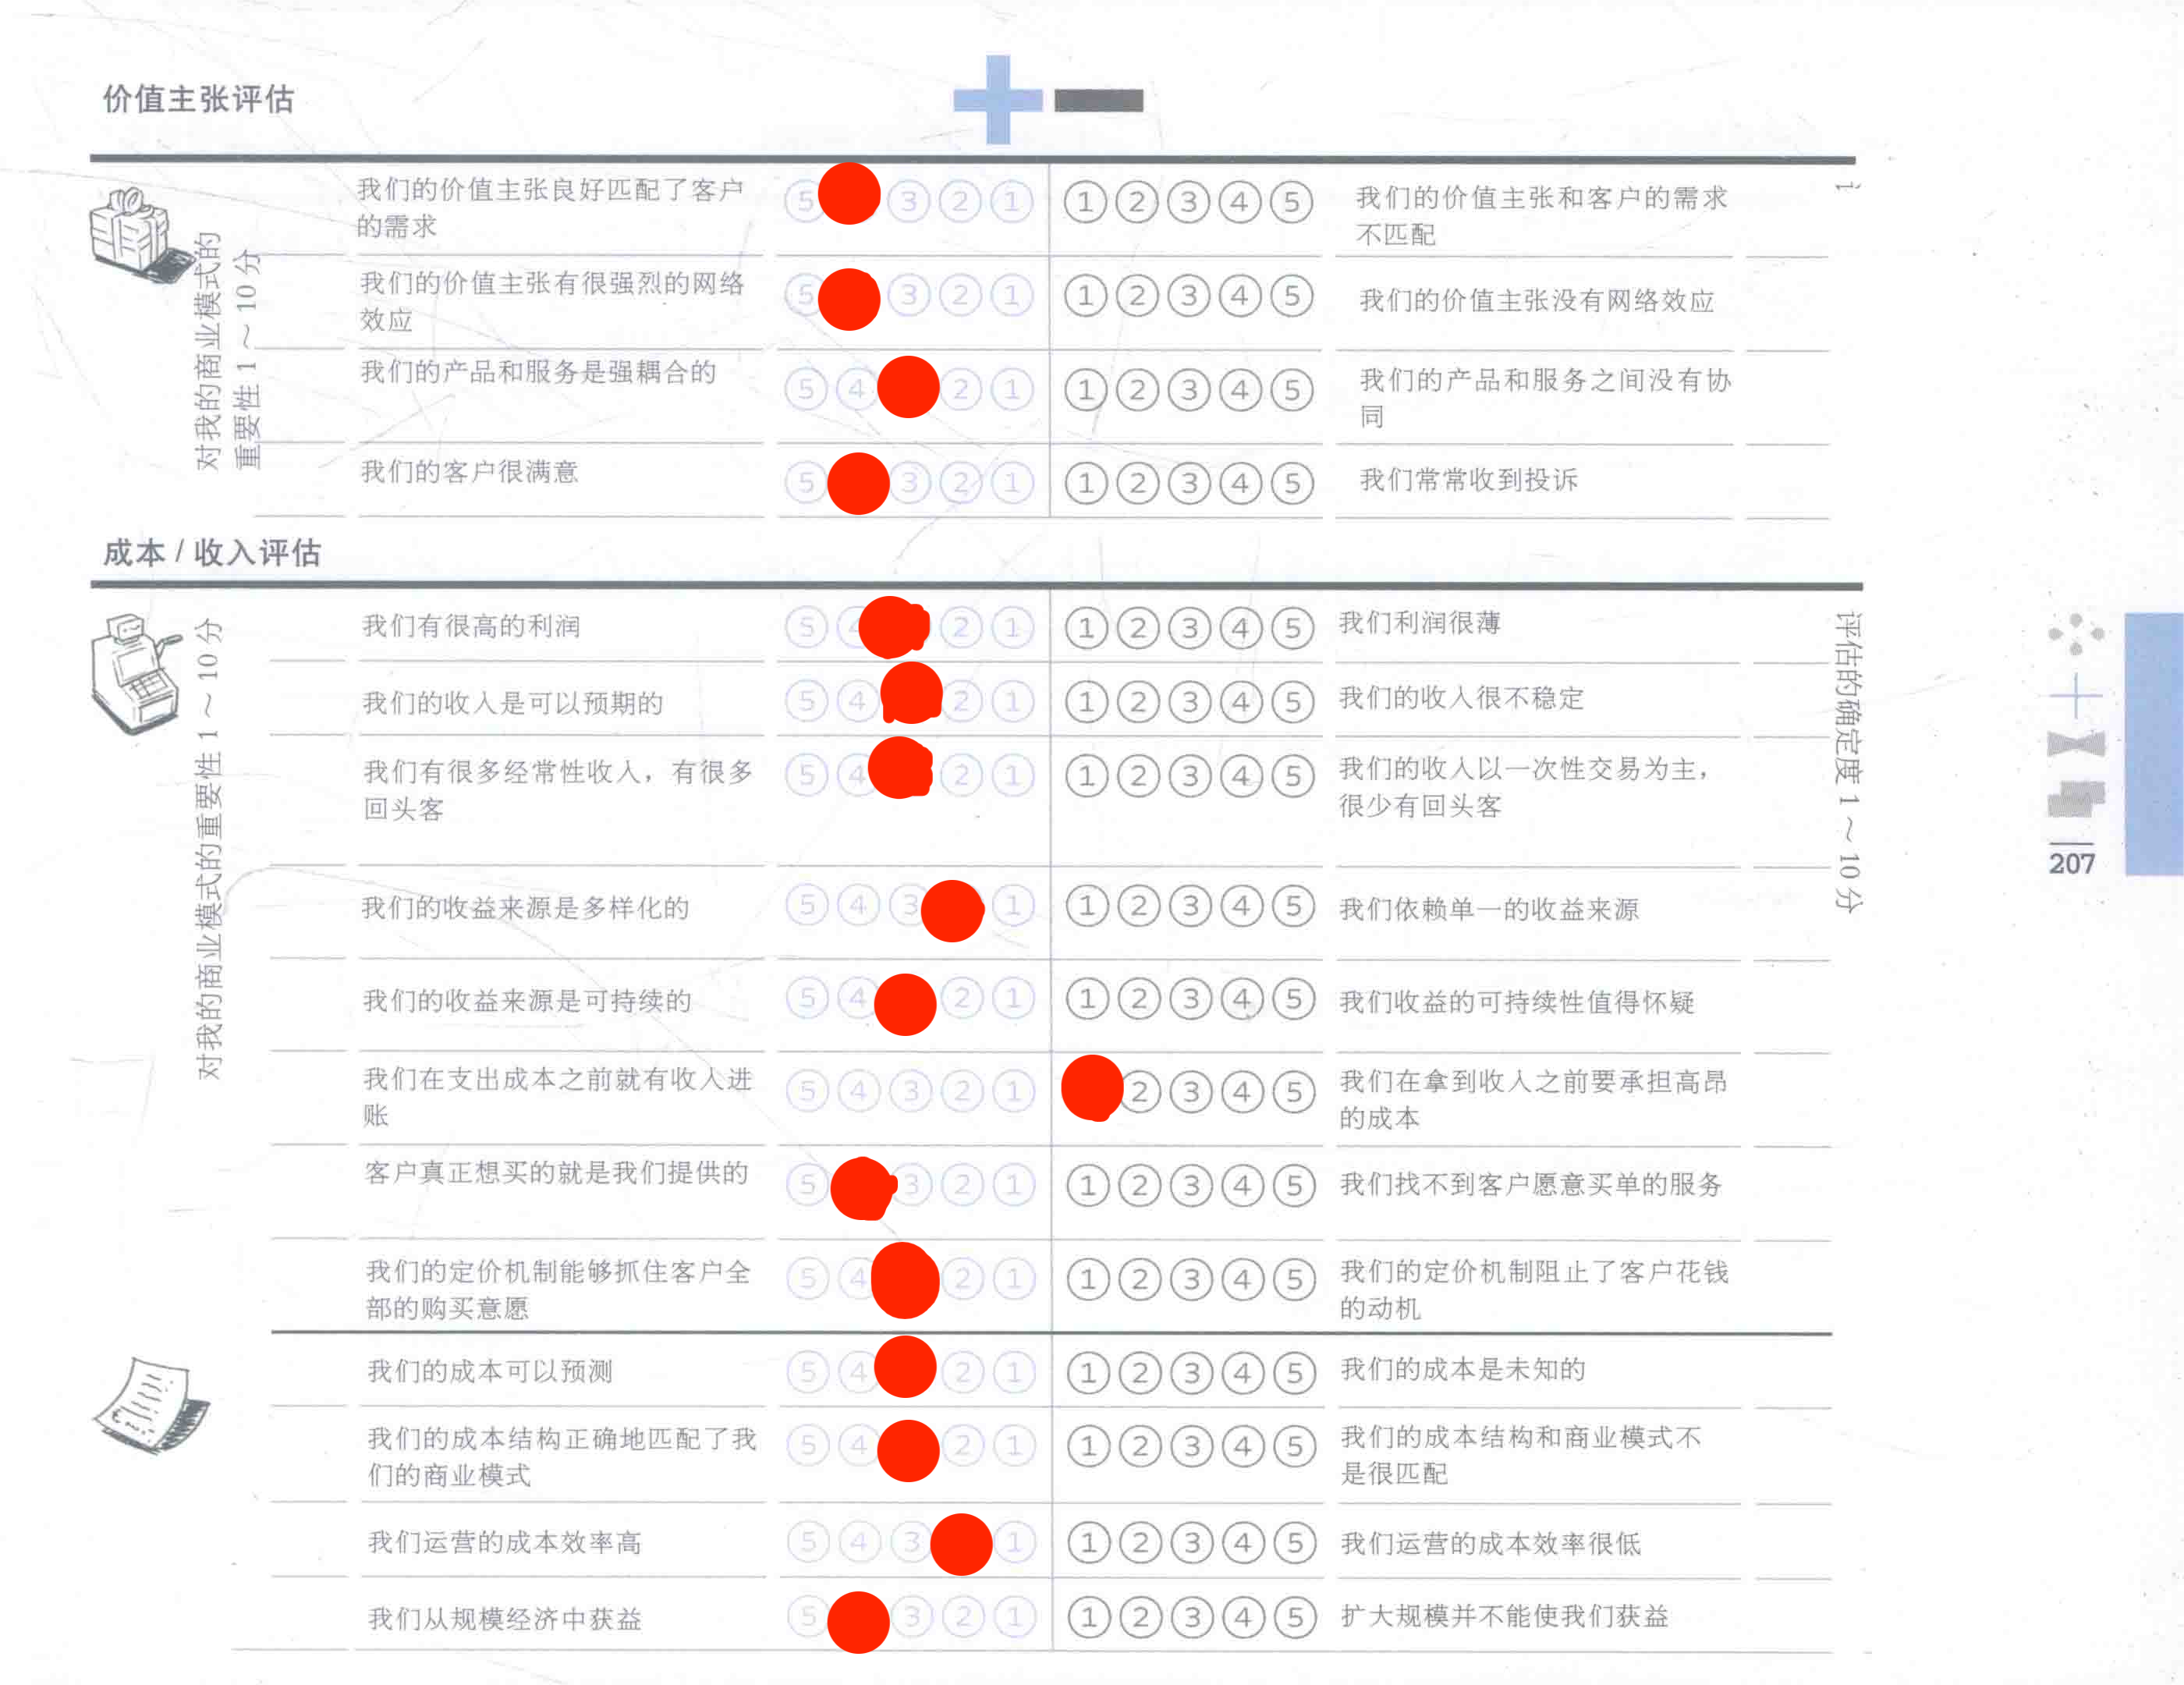
\includegraphics[width=20cm,height=15cm]{png/S&W1}
    \end{figure}
    \begin{figure}[htbp]
        \centering
        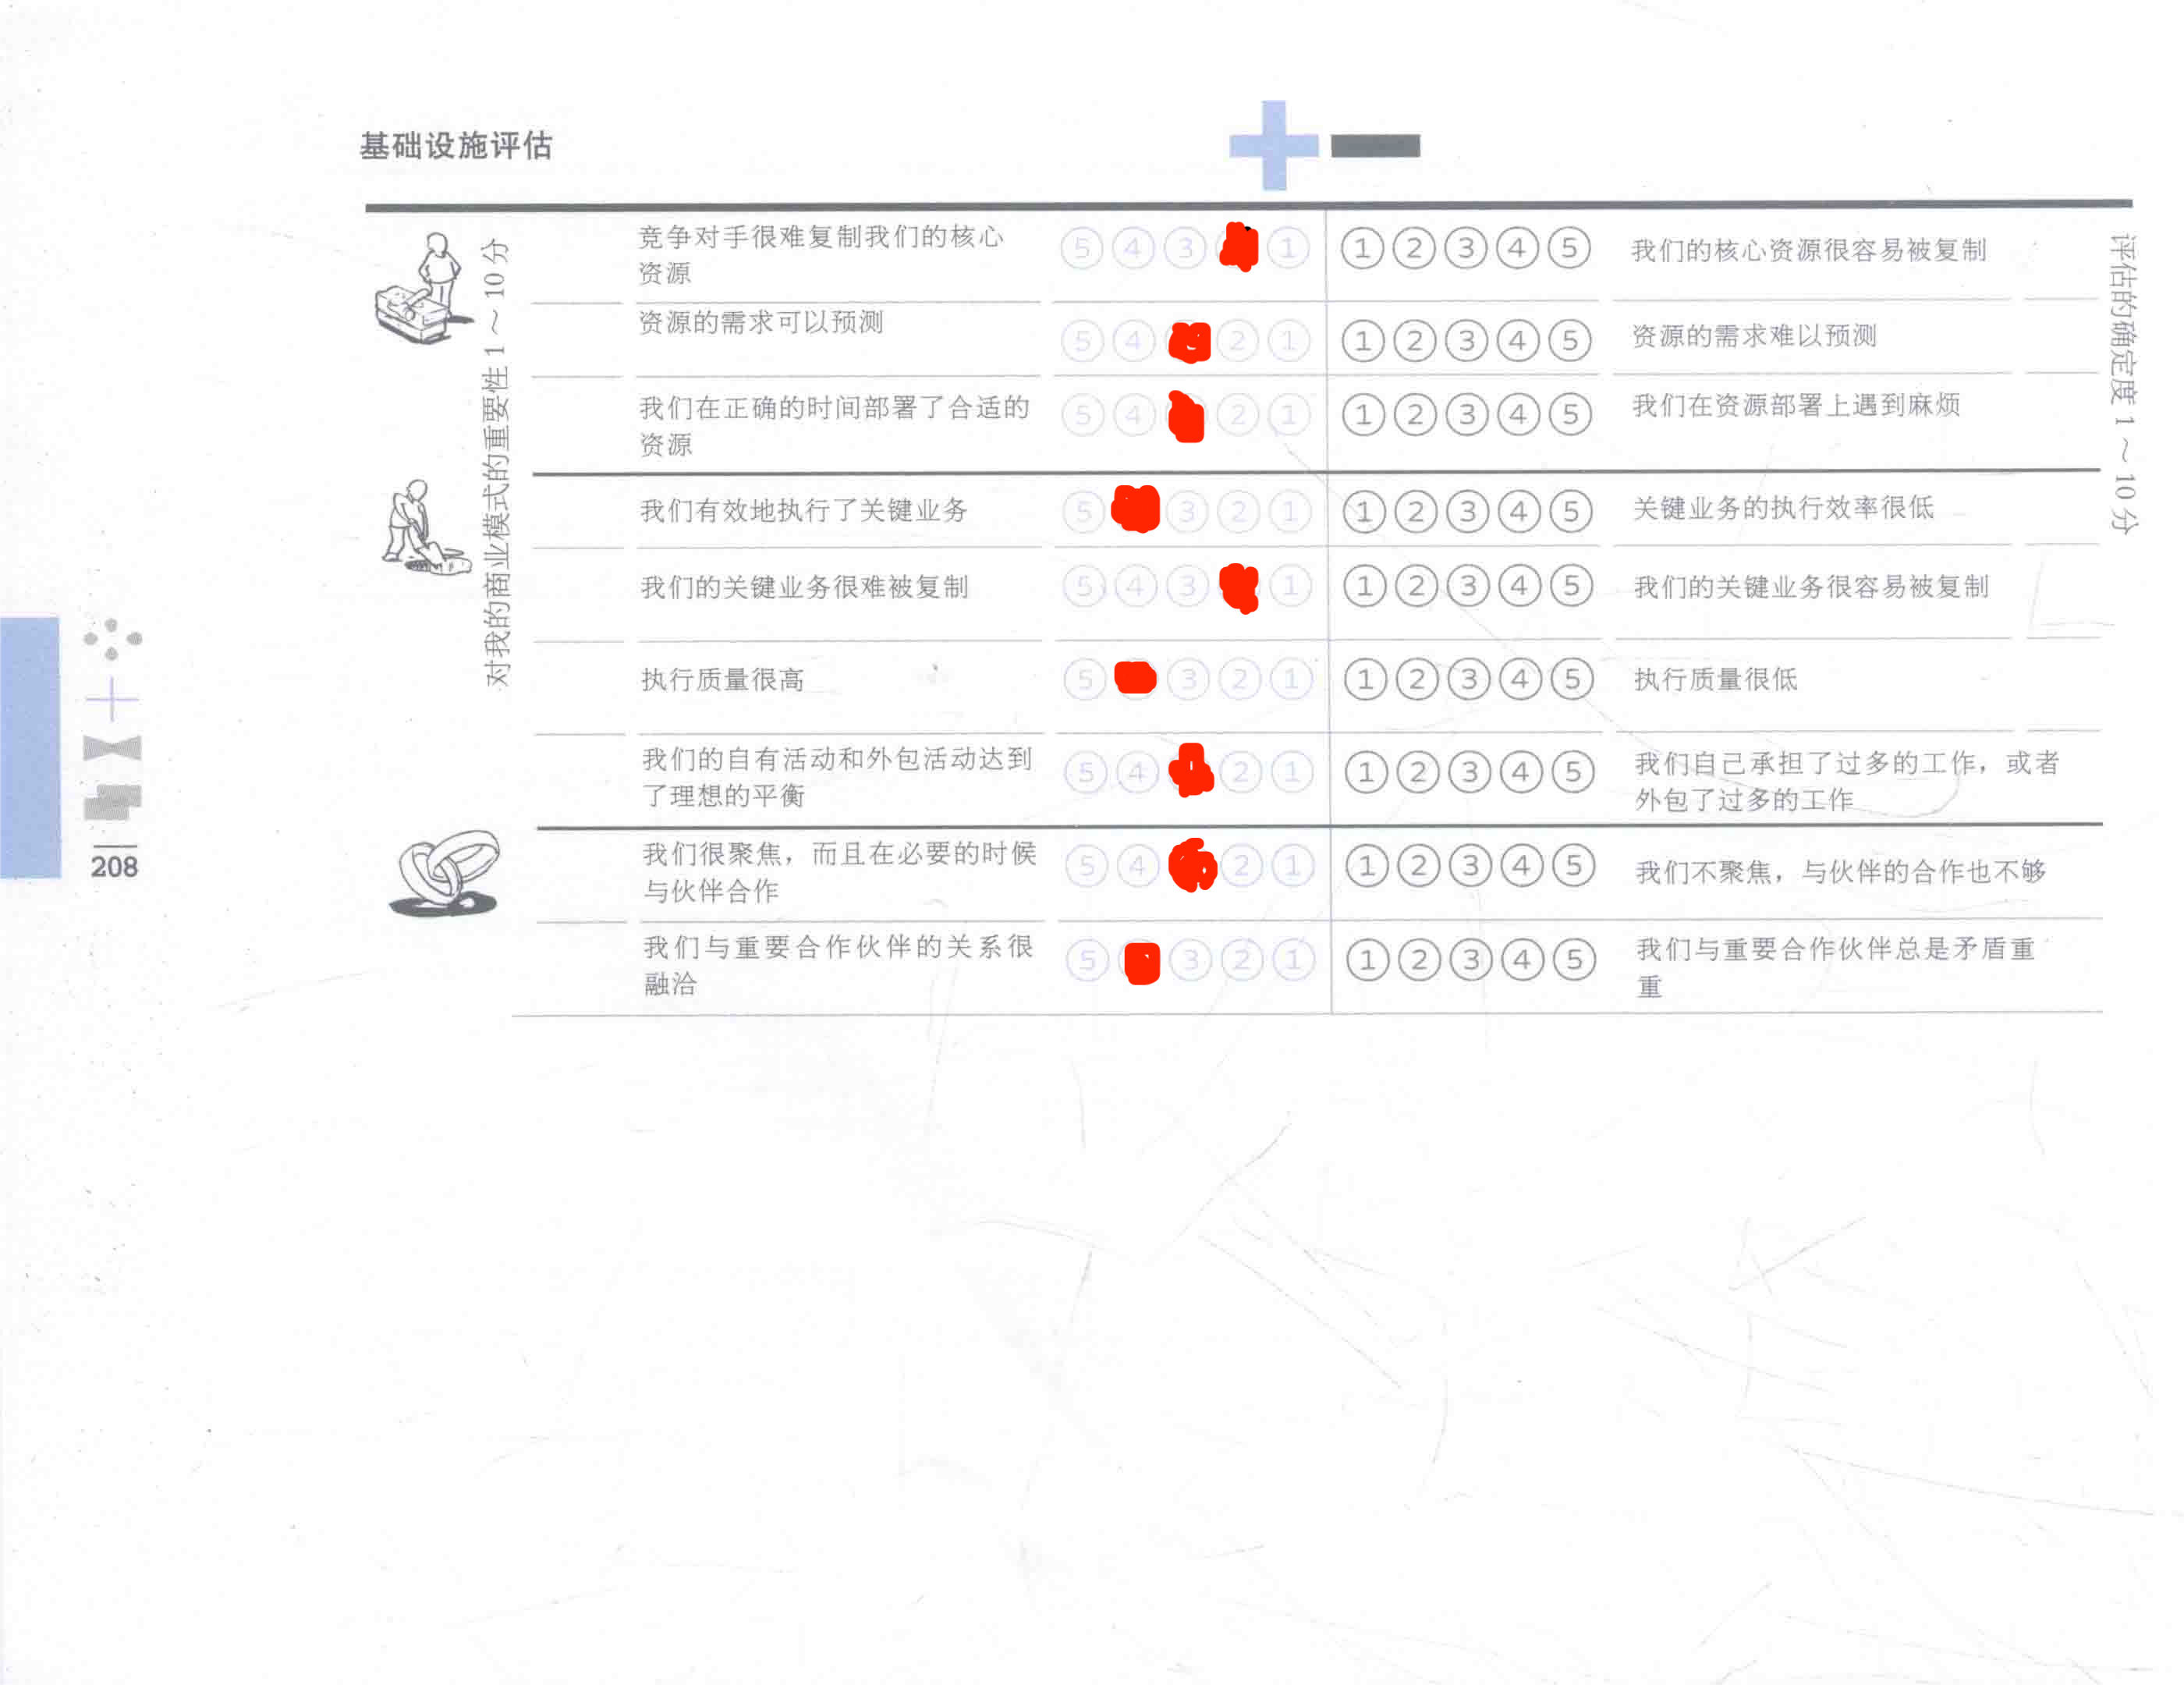
\includegraphics[width=15cm,height=15cm]{png/S&W2}
    \end{figure}
   
    \begin{figure}[htbp]
        \centering
        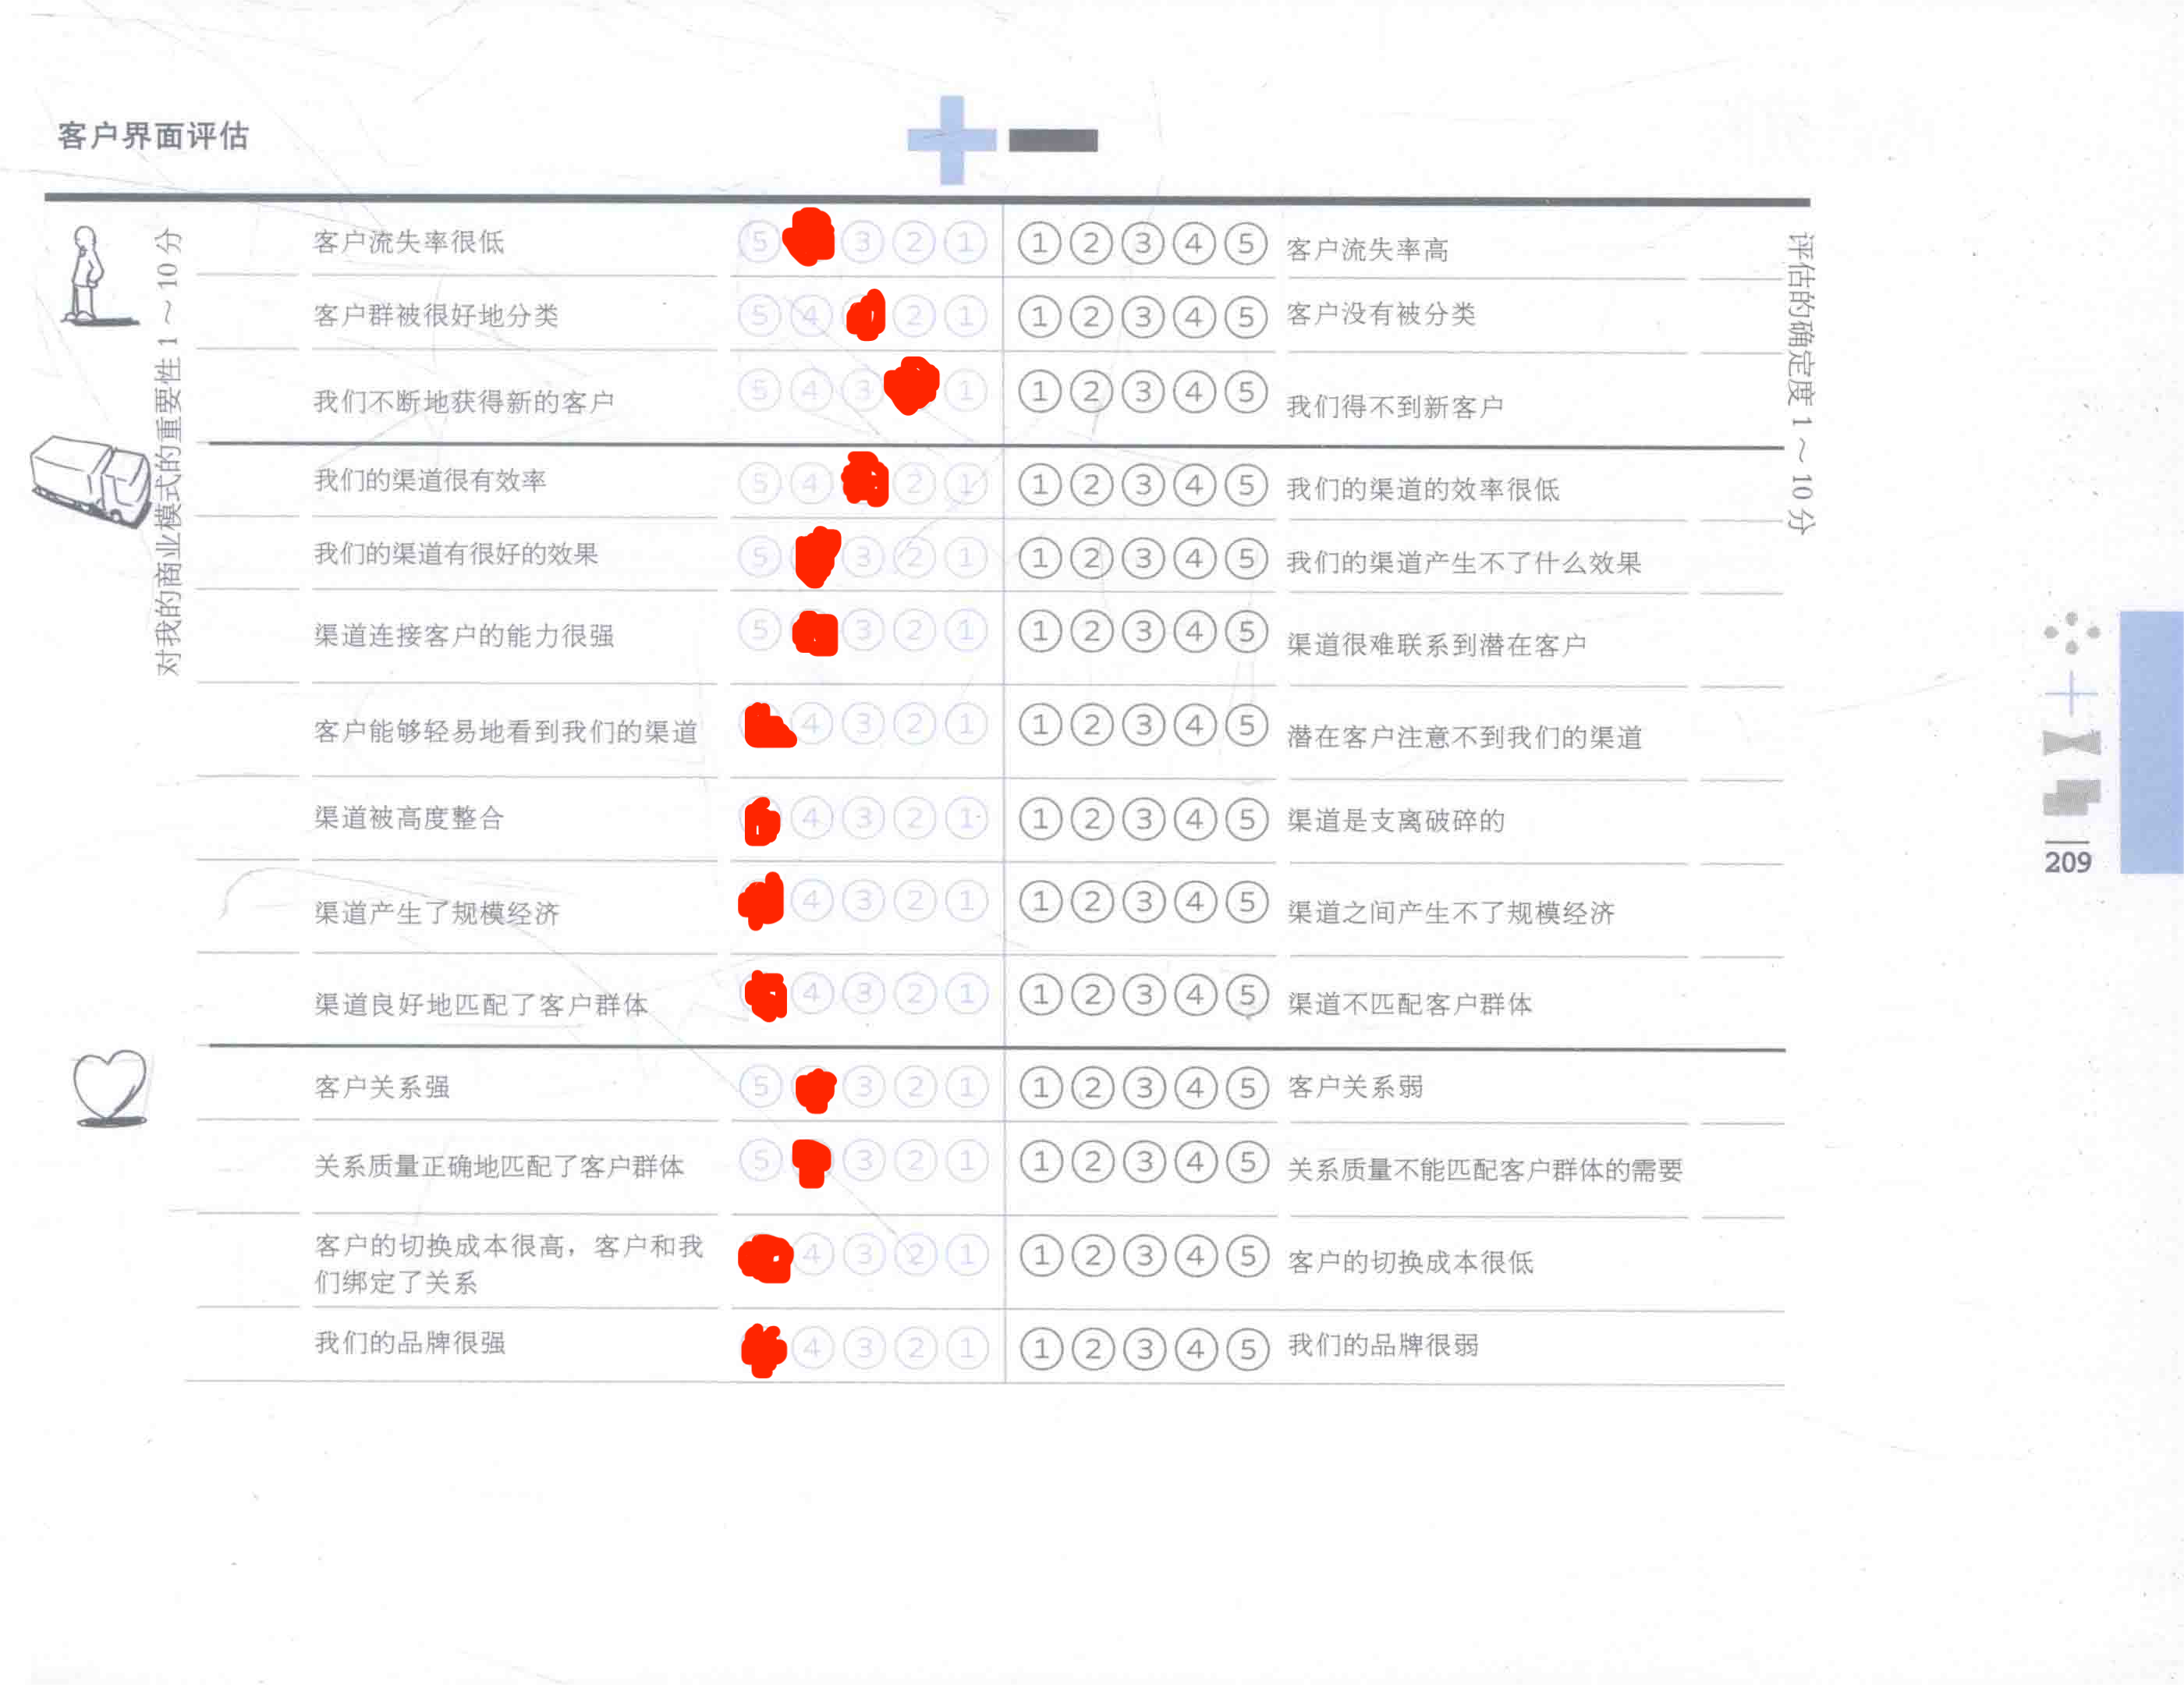
\includegraphics[width=20cm,height=15cm]{png/S&W3}
    \end{figure}
    \clearpage % 强制图片开始新页面
    \subsubsection{价值主张评估}
    \texttt{腾讯会议的独特价值主张}

\begin{itemize}
  \item 腾讯会议产品的价值主张旨在与客户需求紧密契合。他们始终站在客户的角度,深入了解他们真正需要的服务。
  
  \item 提供免费的会议服务,确保普通用户能够轻松享受舒适的会议体验。
  
  \item 为需要更个性化设置、更长时间、更多参会人数以及更大云存储空间等功能的用户提供收费的VIP服务。
  
  \item 面向企业用户提供高级企业会议服务;同时,为学者用户提供专属的“自习室”和网络研讨会议。
  
  \item 始终坚持“对症下药”的原则,以用户为中心,通过收集用户反馈不断优化腾讯会议产品,以满足他们的合理需求。
\end{itemize}

\texttt{腾讯会议的强大网络效应}

\begin{itemize}
  \item 腾讯会议的价值主张具有显著的网络效应。产品的价值取决于使用该产品的其他用户数量,即网络外部性或网络效应。
  
  \item 腾讯会议虚拟会议软件是一个典型的具有网络效应的产品。在刚开始运营时,他们面临高昂的运营成本,并且用户只能与数量有限的人交流信息和使用经验。
  
  \item 随着口碑的积累和知名度的提高,他们将有足够的流水来支付成本并逐渐实现盈利。同时,随着客户数量的增多,像公开会议这种需要大量潜在用户群体的服务也能有效提高腾讯会议产品本身的价值。
  
  \item 因此,腾讯会议的价值主张具有强烈的网络效应。
\end{itemize}

\texttt{腾讯会议的高度耦合产品和服务}

\begin{itemize}
  \item 腾讯会议虚拟会议软件的存在旨在为用户提供仿真实的会议服务。他们追求通过产品为顾客提供最真实、最自然、最愉悦的服务,因此,可以说他们的产品和服务之间存在密切的关系。
\end{itemize}

\texttt{腾讯会议的客户满意度保障}

\begin{itemize}
  \item 他们确信腾讯会议的客户将会非常满意。腾讯会议虚拟会议软件不断追求卓越的用户体验。一旦用户提出不满意的反馈,他们会进行权衡和测试,在经过权衡和测试之后,会做出相应的优化⽅案。
\end{itemize}
\textbf{调研:}
\begin{itemize}
    \item 腾讯会议准备从‘产品的专业能力与体验’进化到‘建设开放生态’,将以更专业、开放的姿态,引入更多的伙伴,更好的服务行业与客户。\footnote{《如何理解腾讯会议3.0“会聚力”的价值主张》}
    \item 腾讯会议企业版将推出混合云部署,混合云部署更加灵活、稳定,能够方便企业管理员的远程运维,更提高了大型企业的使用感受,内部会议可以部署在专有云上,保证信息资产安全。\footnote{《服务3亿用户、14亿场会,腾讯会议企业版迎来重大升级》}
    \item 腾讯会议作为在线办公软件中的一匹黑马,自2019年底发布以来就出现了高速增长,仅仅上线两个月内,每日活跃用户就超过1000万,一举成为中国最多视频会议产品,助力全球抗击疫情。\footnote{《有人给腾讯会议算了一笔账,5个月节约社会成本高达714亿元》}
\end{itemize}
\subsubsection{成本收入评估}
\texttt{腾讯会议较高的利润。}


腾讯会议旗下有众多vip才能享受的服务,这些服务有很多是中大型企业经常甚至必须使用到的,腾讯会议在重视用户体验和口碑的同时,
也会收取相应的费用,对于不经常使用的用户完全可以只使用免费服务即可,腾讯会议的收费功能更多的是面向那些经常要开展大型会议的中大型企业,或者对
线上学术研讨有强烈需求的教育机构等。他们一次会议的人数众多,时间较长,对腾讯会议vip提供的服务有较强的依赖性。他们的vip服务主要分为三个档次:个人会员版、商业版、企业版。针对不同客户都有让他们难以割舍的服务。
腾讯会议的收入基本是可以预期的。在VIP会员费板块,通过引入年卡、连续包月等方式
保证收入的可预期性。同时和教育机构以及高校、企业的合作往往都是长期的,从中收取
的相应的团体专属使用权的购买费用自然是可以预期的。当然,也存在像云存储使用费这
样的可预期性一般的收入,也尽可能的会去通过一次性购买足量的云存储空间给予折
扣的方式来提高其可预期性。\\

\texttt{腾讯会议有很多经常性的收入,有很多回头客的。}腾讯会议提供的VIP服务是具备用户黏性的,他们以用户为中心的主旨会使他们在留住用户这一块有着较强的自信,再加上引入的连续包
月的机制,可以保证收入的经常性。任何回头客都是建立在产品对自己有足够的吸引力之
上的,不断优化的舒适的使用体验是他们最大的竞争力,也是他们留住用户,并从用户群
体中获得经常性收入的保证。其中的会议字幕翻译、实时转译功能对某些跨国企业有非常大的吸引力。\\

\texttt{腾讯会议收入形式是单一的,但来源于多样的群体。}腾讯会议有单一的收入形式,即增值服务收入。多样的付费群体包括:个人VIP用户,支付VIP服务费,教育机构、高校与企业支付相应的团体专属使用权的购
买费用,对有拥有更大的云存储空间的需求的用户支付云空间按存储字节的收费,还包括各群体临时增加会议时长的费用。\\

\texttt{腾讯会议的收入是可持续的。}正如前面所说,腾讯会议提供的VIP服务是具备用户黏性的,合理的价格
并且绝对舒适的使用体验,有大量实用的服务功能,可以让用户难以脱离使用VIP服务。\\

\texttt{腾讯会议拿到收入之前实际上要承担较为高昂的成本。}产品软件的制作本身是需要投入大量的成本的,再加上腾讯会议对用户舒
适实用体验的追求,势必会有更大的研发支出。再加上在产品投入市场的初期,是需要通
过大量广告宣传的方式来增加知名度、吸引用户的,他们所要支付的广告费也是价格不菲
的。而且维护用户数据的大型数据库的租用或者购买、分布式系统的部署、运行服务的服务器,这些都是非常大的成本。
因此在拿到收入之前实际上整体是要承担较为高昂的成本的。\\

\texttt{客户真正想买的就是腾讯会议提供的产品和服务。}腾讯会议是以用户为中心的,他们重视用户的使用体验和口碑的积累,即使是对普通的用户也会给予他们足够舒适的使用体验,这些是为普通用户提供的。个性化设置、更长会议时间、更多大参会人数、
更大的云存储空间等,他们提供VIP服务的购买,这些功能对某些对远程会议有粘性需求的企业、个人都是非常有吸引力的,而且还会根据用户的反馈来进行优化整改。
腾讯会议的定价机制基本能够抓住客户的购买意愿。腾讯会议大致上分了三类vip用户:个人会员版、商业版、企业版。个人版30元/月具有更丰富的虚拟背景、会聚模式场景、自动会议纪要、实时转写等功能。单场会议最高可容纳100/300/500人,可同时开启视频人数为60/300/500人,可根据规模做选购。
商业版4788元/年起,中小企业可以选购腾讯会议商业版,商业版提供最高2000人会议室、200G的云录制空间、直播功能、可视化数据分析、会管会控能力等功能,满足企业日常管理的需求。
企业版有较大的灵活性,企业版有更强大的协作、会管会控及企业会议管理能力,最高2000人会议室、无限云录制空间、企业仪表盘等功能,并基于API无缝与企业业务系统融合。具体价格根据企业选定服务。\\

\texttt{腾讯会议的成本在一定程度上是可以预测的。}
腾讯会议的成本包括带宽和服务器成本、运营成本以及附加功能收费等。
腾讯会议需要承担高昂的带宽和服务器成本。视频会议需要大量的数据传输和存储,因此需要高速的网络和强大的服务器来支持。这些成本对于腾讯会议来说是非常高昂的,尤其在用户数量激增的情况下,服务器和带宽的需求也会相应增加。
腾讯会议还需要承担运营成本。除了服务器和带宽成本之外,腾讯会议还需要支付员工工资、市场营销、技术支持等方面的费用。这些成本也是非常高昂的,尤其在竞争激烈的市场环境中,腾讯会议需要不断投入资金来保持领先地位。
腾讯会议通过收取附加功能费用来弥补成本。腾讯会议提供了一些高级功能,例如云录制、同声传译等,这些功能需要额外的开发和技术支持成本。腾讯会议通过向用户收取这些功能的费用来弥补成本。
腾讯会议成本结构基本可以匹配他们的商业模式。\\
1.免费使用:腾讯会议的基础功能免费提供给用户,这有助于吸引大量用户,从而形成网络效应。\\
2.付费增值服务:腾讯会议提供付费的增值服务,如更高质量的视频和音频、更长的会议时间、更多的会议参与者等。这些服务可以满足不同用户的需求,提高用户体验。\\
3.跨平台支持:腾讯会议支持多种设备,如PC、手机、平板等,方便用户随时随地参加会议。\\
这些特点使得腾讯会议的成本结构可以匹配多种商业模式,具体来说:\\
1.免费+广告模式:腾讯会议可以通过在免费版本中投放广告来获得收入。这种模式适用于那些希望通过广告宣传自己的品牌和产品的公司。\\
2.付费订阅模式:腾讯会议可以通过提供付费的增值服务来获得收入。这种模式适用于那些需要更高质量服务的用户,如企业用户。\\
3.合作伙伴模式:腾讯会议可以与其他企业合作,提供定制化的远程会议解决方案。这种模式适用于那些需要特殊功能的用户,如政府部门、金融机构等。\\

\texttt{腾讯会议运营的成本效率相对较低。}腾讯会议一年的运营成本至少大几十个亿。 而腾讯会议几年来的营收非常有限,仅有数亿元规模。 这对于大几十亿的成本,可以说杯水车薪。
腾讯会议是要从规模经济中获益的。规模经济是企业产品绝对量增加时,其单位成本下降。
通俗的来说就是扩大经营规模可以降低平均成本,从而提高利润水平。这其实就是他们的主
要盈利模式,他们开发最初版本的成本是他们成本的大头,他们只有在拥有了足够的用
户,并从他们身上获利之后,才能降低他们的单位成本,也就是“摊薄”成本,从而他们的
利润也会在用户规模不断扩张的过程中不断的增长、提高。\\
\textbf{调研:}
\begin{itemize}
    \item 腾讯会议是一款月活跃用户过亿的在线办公软件,他拥有庞大的年轻的、高质量用户群体,他积极运用其广告能力,能够帮助广大品牌深度触达办公场景人群,凭借更沉浸式的互动广告玩法,有效解决“吸引消费者注意力”难题。\footnote{《腾讯会议如何盈利?》}
    \item 受疫情影响,企业数字化转型迫在眉睫,使得轻量化SaaS服务快速普及:腾讯会议、腾讯企点和企业微信等应用都在去年实现了较高速度增长。\footnote{《腾讯2020年财报:腾讯会议跻身中国No.1,加速提升市场渗透率》}
    \item 腾讯会议开放了覆盖会议邀约、会中管理、会后沉淀等相关功能超 300 个 API 接口,数千家企业组织基于腾讯会议开放提供的 API 接口,进行商业会议讨论,日均调用次数过千万。此外,腾讯会议合作伙伴已超过了 300 家,比去年增加了 2 倍有余,今年上半年腾讯会议代理收入同比增长近 200\%。\footnote{《用户突破 4 亿!腾讯会议接入混元大模型》}
\end{itemize}




    \subsection{评估威胁}\label{subsec:threat}
    \subsubsection{打分结果}
    \begin{figure}[htbp]
        \centering
        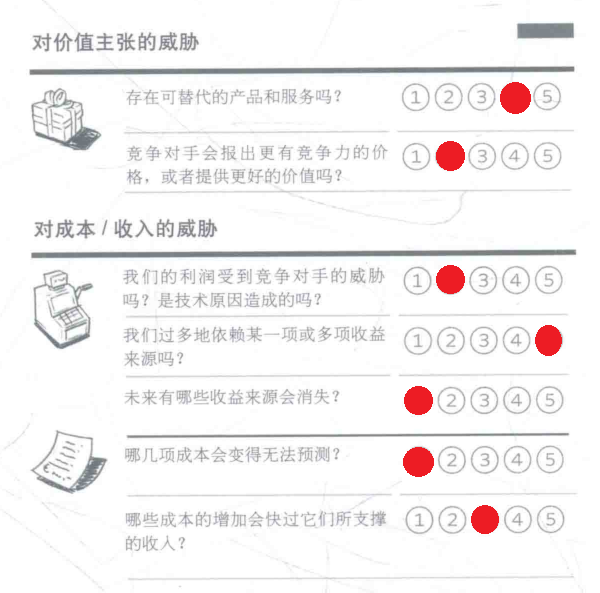
\includegraphics[width=15cm,height=15cm]{png/评估威胁}
    \end{figure}
    \clearpage % 强制图片开始新页面

    \subsubsection{价值主张评估}


    1.
    当前市场上确实存在有腾讯会议的代替产品,如国外的 Skype 和 Zoom,国内的钉钉、华为云会议、飞书等。
    尽管据 iResearch 调研,腾讯会议在疫情中崛起成为国内使用量最大的视频会议软件之一,
    \footnote{https://www.iresearch.com.cn/Detail/report?id=3605\&isfree=0}
    但不可否认,市场上仍有许多软件能提供腾讯会议所提供的价值主张,这使得腾讯会议面临较大的被替代威胁


    2.
    腾讯会议的竞争对手不太能给出更有竞争力的价格或服务。
    我们分别从华为云会议、钉钉、Zoom 以及腾讯会议的官方网站上获取了这些产品的报价和对应功能。
    首先,它们均采用了免费增值的商业模式,均提供基础免费功能。
    在增值服务方面,
    华为云会议提供了250¥/月(3000¥/年)的标准版服务和350¥/月(4200¥/年)的旗舰版服务。
    \footnote{https://www.huaweicloud.com/product/meeting.html}
    钉钉给出了最高的报价:9800¥/年的专业版服务、98000¥/年的专属版服务以及定制的专有版服务。
    \footnote{https://pages.dingtalk.com/wow/z/tianyuan/default/opportunity\_index?spm=a213l2.13146415.0.0.7f1571e1F3EIGn}
    在国外流行的Zoom反而提出了远远低于上述软件的报价:149.90\$/年的专业版,199.90\$/年的商业版,以及更多的定制服务。
    \footnote{https://zoom.us/zh-cn/pricing}
    对比上述三家,腾讯会议面向个人的有 98¥/月(1176¥/年)、 499¥/月(5988¥/年)、999¥/月(11988¥/年),面向企业的有4788¥/年等报价,此外更多详情请阅腾讯会议官网。
    \footnote{https://meeting.tencent.com/buy/index.html?mid=web.p.topdh.djygm}
    综上,腾讯会议提供了多种层次的不同价位服务,其报价与功能与同行相比较也算适中,难以被同类产品从价格和价值方面威胁。


    \subsubsection{成本/收入评估}
    1.
    腾讯会议的利润几乎不会受到竞争对手的威胁。其原因已经提过:腾讯会议在疫情发生后,迅速占领了国内市场的大量份额成为国内的主流视频会议软件。
    除非再发生一次能培养出更大的行业市场的事件,或行业中有革命性的软件出现,否则腾讯会议的营收很难被其他同类软件抢走。
    并且,腾讯会议是下属于腾讯的产品,腾讯旗下还有微信、QQ等流行应用。腾讯会议依靠腾讯资金、技术、应用生态链和用户数量,是较难被同类产品威胁到利润的。


    2.
    尽管 SW 分析中我们说腾讯会议的收益来自多种群体,但归根结底腾讯会议依赖于单一的收入形式:增值服务收费。
    我们从腾讯的2022年度报表中可以看出增值服务是腾讯的主要收入来源,其占总收入的百分比为52\%,而金融科技及企业服务占31\%,广告收入占16\%。
    \footnote{https://static.www.tencent.com/uploads/2023/04/06/eac54c79c67d8a501bc4b65ff1718223.pdf}
    一方面,当今的办公软件注重于提高用户的办公效率,很少投放广告。
    腾讯会议的纯办公软件性质决定了它几乎没有可投放广告的位置。
    腾讯会议也绝不能窃听、收集会议信息以定向投放广告,这是违法的。
    也就是说,腾讯会议仅能在少数界面,例如启动界面,投放少量商务办公广告来获取少量广告收入。
    另一方面,腾讯会议软件本身要追求简单易用以吸引用户,除了一些企业定制场景外,提供技术支持服务营收的机会也不多。
    综上,增值服务仍是腾讯会议依靠的主要收入来源。


    3.
    腾讯会议未来可能会出现收益缩减,但不会出现收益来源会消失的情景。
    我们提到过:腾讯会议是免费增值商业模式,以增值服务作为主要收益来源。
    在这种情况下,腾讯会议的收益缩减主要有两种可能:
    一是市场产生一定程度的萎缩,付费用户减少,市场萎缩可能来源于随着疫情结束等因素,从 iResearch 的调查报告中可以看到腾讯会议的下载量在后疫情时代确有所下降。
    二是市场上出现革命性的新产品,抢占腾讯会议市场份额,腾讯会议确实有较多的替代产品,但目前没有革命性产品来抢夺份额。
    综上,增值收费在近未来可能会缩减,但它作为腾讯会议的核心收入,只有腾讯会议彻底消亡才会消失。


    4.
    腾讯会议发展至今,成本结构基本确定。
    第一,腾讯会议已开发完毕,开发成本已确定;
    第二,腾讯会议已度过疫情初期的使用高峰,进入了稳定部署维护的阶段,运行维护成本、设备成本等成本的峰值已被掌握。/;
    第三,腾讯会议已打出名气,宣传成本不会再增加。
    不出意外的话,腾讯会议不会再遇到不可预测的成本。

    5.
    特殊情况下,腾讯会议的运维成本可能迅速增大,超过软件本身带来的的收入。
    例如,在疫情爆发后,线上办公需求井喷式增长。根据腾讯科技讯介绍,当时腾讯会议为满足市场需求,在8天内增加大量的云主机和计算资源。
    \footnote{https://new.qq.com/rain/a/TEC2020020600971700}
    与此同时,腾讯会议向大众免费提供了视频会议服务,而没有收取增值费。
    这样的策略,为腾讯会议吸引了大量的用户但却没有带来收入,反而使得腾讯会议的运维成本剧增。
    尽管腾讯会议的成本收入数据未被公布,但是观察同类产品 Zoom 在同一时间段的率也仅有 3\%。
    \footnote{https://quotes.sina.com.cn/usstock/hq/income.php?s=zm\&t=annual}
    由此推测,腾讯会议在疫情初期的运维成本迅速增加,却缺乏足够的收入,出现了成本超过收入的情况
    尽管类似情况再发生的概率不大,但威胁确实存在。

    \subsection{评估机会}\label{subsec:opportunity}
    \subsubsection{打分结果}
    \begin{figure}[htbp]
        \centering
        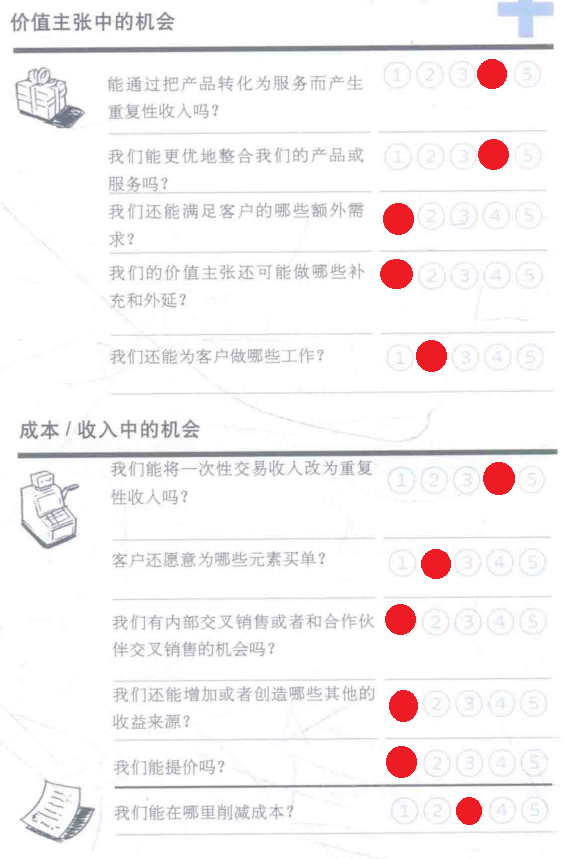
\includegraphics[width=12cm,height=18cm]{png/评估机会}
    \end{figure}
    \clearpage % 强制图片开始新页面


    \subsubsection{价值主张评估}


    1.
    我们在分析腾讯会议定价时论述过,腾讯会议不是买断式的软件,而是以月租、年租的形式收取增值服务费。
    此外,腾讯会议还提供了所谓的“腾讯会议 SaaS 版新购”的服务购买方式。
    \footnote{https://buy.cloud.tencent.com/tm}
    因此我们得出结论: 腾讯会议已通过提供服务的方式获取重复性收入。


    2.
    在整合产品和服务方面,腾讯还有改进空间。
    理由如下:目前腾讯会议可以通过QQ、微信账号进行登录,产品之间进行了一定程度的整合;
    但腾讯还可以进一步整合,例如将腾讯会议等产品的入口嵌入QQ、微信等腾讯旗下的其他产品中,形成一个联系更紧、整合程度更深的应用生态链,将QQ、微信上的庞大用户群引向腾讯会议。
    这样既能方便用户享受腾讯的应用服务生态链,又能借助该生态链牢牢吸引用户。


    3.
    我们认为,基本已经没有额外的客户需求可供腾讯会议发掘。
    除了基本的视频服务,腾讯会议还提供了包括共享桌面、文字图片聊天室、AI识别的服务,与在线会议有关的服务已经趋于全面。
    除非创造新的价值主张,否则强行添加更多功能,反而既增加了成本,又使得应用变得冗余臃肿。


    4.
    正如我们上文分析分析所说,腾讯会议专注于视频的价值主张已基本没有补充和外延的机会。
    腾讯会议应该考虑的是,从深度方面优化已有价值主张(例如当前会议室安全性不足),或是创造新的价值主张(例如创造开放广场)


    5.
    尽管我们认为腾讯会议的价值主张基本没有横向扩展的空间了,但腾讯会议仍可以为原价值主张方面提供更优服务。
    例如,腾讯会议可以优化性能,提高网络吞吐量、降低硬件占用率,提供更精准的语音识别服务、自动生成字幕功能等,提高用户的使用体验。
    此外,腾讯会议的会议室ID和密码的入会方式也不够便利和安全。
    综上,腾讯会议还有进一步优化已有功能以提高客户使用体验的空间。


    \subsubsection{成本/收入评估}


    1.
    腾讯会议的重复性收入问题我们已进行详细的讨论,请见 4.3.2.1。


    2.
    在评估价值主张的机会评估中我们提及,假如腾讯会议能深度优化应用以提高应用体验,或许能吸引更多的用户买单。
    目前腾讯会议的 AI 精确度仍有待提高,会议安全性和便利性也不足,通过分享会议ID和密码方式入会可能出现陌生人闯入会议室的情形。
    将这些方面完善,或许能吸引更多用户买单。


    3.
    腾讯会议内部销售的意义不大,有一定的向合作伙伴销售的可能。
    腾讯企业内部的会议需求,大部分都可以通过面对面会议解决,当有远程会议需求时也应该免费向内部员工提供腾讯会议服务,让企业内部人员为本公司开发的办公工具买单是荒诞的行为。
    对于有特殊在线会议需求的合作伙伴,腾讯会议可以尝试提供定制化的远程会议解决方案,不过这并没有交叉销售的必要,完全可以通过市场销售直接进行。


    4.
    正如上文所述,增值服务是腾讯会议的最主要的收入来源。
    除非能创造新的价值主张,否则在当前网络会议的市场需求不再扩大的情况下,腾讯会议难以获得更多增值费。


    5.
    腾讯会议提价的空间不大。
    在市场上仍存在很多替代产品,且客户可以转向线下会议的情况下,腾讯会议再提价很可能造成客户流失,反而可能造成总收入下降。
    在市场均价没有上升之前,或腾讯会议没有大幅优于其他产品之前,腾讯对于提价行为必须足够谨慎。

    6.
    腾讯会议确实有不少的降低成本空间。
    我们前文提过,腾讯会议的主要成本在于大量的算力资源成本和运维成本。
    优化算法、优化代码结构、适当减少向免费用户提供的服务、删减不必要的服务等方式,都有可能降低运维成本。

    
    \section{蓝海战略}

    
    \subsection{选择从价值主张探讨的理由}
    基于前文对竞品腾讯会议的总体评估及 SWOT 分析,我们认为腾讯会议围绕“提供便利的、可定制的在线视频会议服务”这一价值主张,已开展了优质的业务活动,
    并且支持这一价值主张的成本结构可预测、与商业模式较为匹配,价值主张也成功地通过Web平台、QQ和微信链接等渠道交付给用户。
    也就是说,腾讯会议的商业模式已经是一个成熟、稳定的商业模式。
    因此,本小组的创意需要通过根本性的差异化来创造新的行业,避免在原商业模式内与腾讯会议直接竞争。
    为此我们聚焦于提供差异化的价值主张,由差异化的价值主张来实现新价值的创造与旧成本的缩减。
    新价值主张的具体内容,正是我们在第一阶段的创意中所提到的社交系统、会议的开放性与私密性设置和会议的高互动性。
    
    \subsection{蓝海战略探究结果的画布}
    \textbf{以下是对本小组创意与竞品腾讯会议对比分析后所作的蓝海战略商业模式画布}
    \clearpage
    \begin{figure}[htbp]
        \centering
        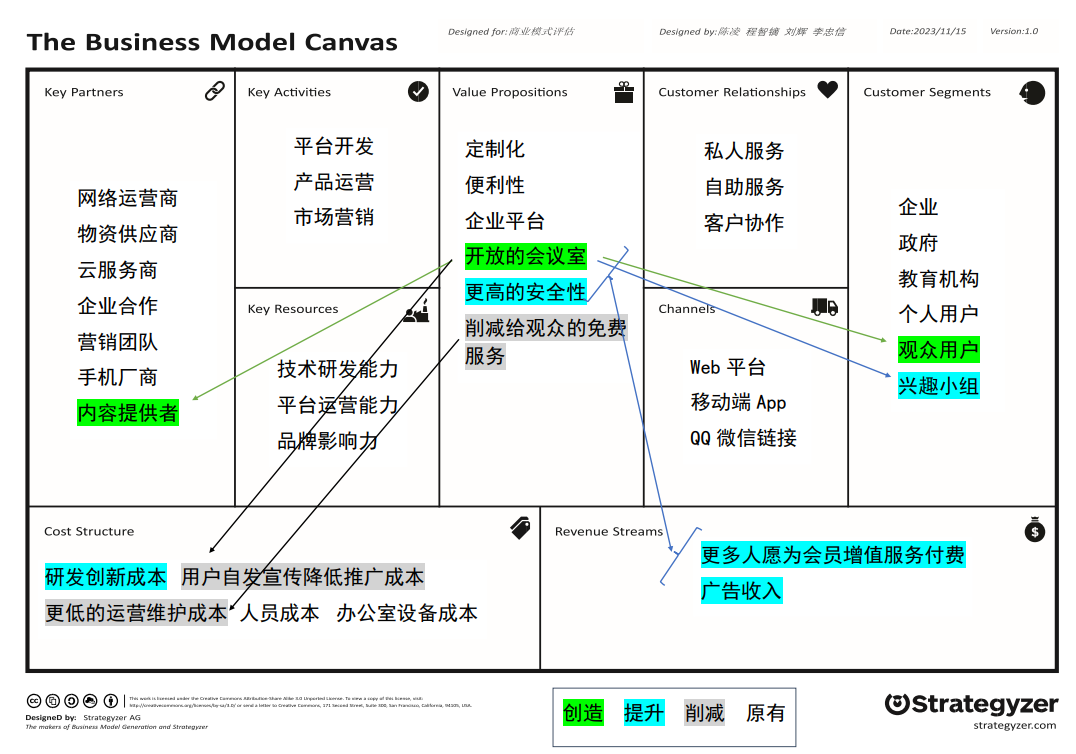
\includegraphics[scale=0.4]{png/蓝海战略}
        \caption{}
    \end{figure}


    \subsection{基于蓝海战略四项行动探究的论述}
    \subsubsection{创造}
    我们发现腾讯会议在“定制”和“便利”上,仍有更多价值主张值得深度挖掘。
    首先,是“开放性”和“便利性”不足。在对腾讯会议的实际使用中,我们发现腾讯会议的所有在线会议室都是通过输入会议室ID及密码(可选)进入。
    此外,腾讯会议的会议室ID及密码必须要通过第三方途径分享,例如通过QQ、微信等方式向与会成员分享。
    究其原因,腾讯会议没有独立的社交系统和独立的通讯录功能,必须依赖其他途径邀请入会。


    为此,正如我们在《项目启动》所说,我们计划创造的新价值主张有以下两点内容:
    其一,是开放广场功能。首先我们让用户可以定制开放的会议室,然后这些会议室可以在“广场”上被其他用户找到并加入。
    开放广场这一价值主张,可以满足各类注重会议室开放性的用户的需求,例如公开课、公开研讨会、娱乐兴趣小组等。
    这也有助于将我们的创意打造为成多边平台商业模式。
    其二,是在创意中引入独立的联系人系统。会议软件本身即带有联系人列表、群组等功能,用户可以直接邀请联系人或某个群组入会,而不必再通过第三方链接邀请入会。
    这不仅能较大程度地提高用户开会的便利程度,而且也能为我们即将提到的“安全控制”功能打基础。

    \subsubsection{提升}

    腾讯会议通过会议室ID及密码参与会议方式,存在着安全性、私密性隐患。
    据《民生周刊》报道,腾讯会议曾出现过所谓“网课入侵”现象,即会议ID及密码暴露、大量无关人员闯入在线会议室进行各种捣乱行为。
    \footnote{https://new.qq.com/rain/a/20221106A02M8M00}
    在网络论坛上,我们也可以看到有不少群众提到了亲身经历的会议室被“入侵”的事件。
    \footnote{https://www.zhihu.com/question/380514759}
    腾讯会议针对这些现象也做出了改进,但我们认为这些改进仍不充分。
    在腾讯会议的 PC 版软件中,对入会权限的控制只有“一刀切”的锁定会议室功能,以及需要主持人较多操作的“等候室”功能。
    \footnote{信息来源于对腾讯会议软件 PC 版的实际使用,软件链接:https://meeting.tencent.com/}


    对此,我们的解决方案是,通过“联系人”功能提升会议的安全控制能力。
    我们计划了引入联系人系统,此时我们的会议可以选择只允许被邀请的联系人入会,这样就可以从根本层面解决陌生人“会议入侵”问题。
    同时,我们还可以提供让未被邀请的人申请入会的功能,是否开启这样的功能由会议主持人决定。


    \subsubsection{削减}
    在腾讯会议的免费增值商业模式中,有大量的用户只是会议观众,而不是会议主持人。
    定制会议的服务,对于大部分的观众型用户并没有太多吸引力,只对少部分主持型用户有吸引力。
    从腾讯会议官网也可得知免费用户的权益已经被削减了。
    \footnote{详情请查看腾讯官网:https://meeting.tencent.com/m/magic-act/5szgxcha4is61qf16uxikfq589/index\_index.html?ovscroll=0\&page=index\&\_\_no\_magic\_qrcode=1}

    假如我们的社区广场能成功吸引足够数量的内容提供者,那么就会出现更多的只对内容感兴趣的观众型用户。
    因此,我们认为可以适度地削减提供给免费用户的创建、定制会议的服务,只提供基础的、容量较小的免费创建会议服务。


    \subsubsection{删除}

    竞品腾讯会议所提供的价值主张基本都围绕着提供优质视频会议服务,它几乎没有其他价值主张。
    因此,我们将不会删除腾讯会议目前所提供的价值主张。


    


\section{更新过的商业模式画布}
    \subsection{更新后的画布}
    \clearpage
    \begin{figure}[htbp]
        \centering
        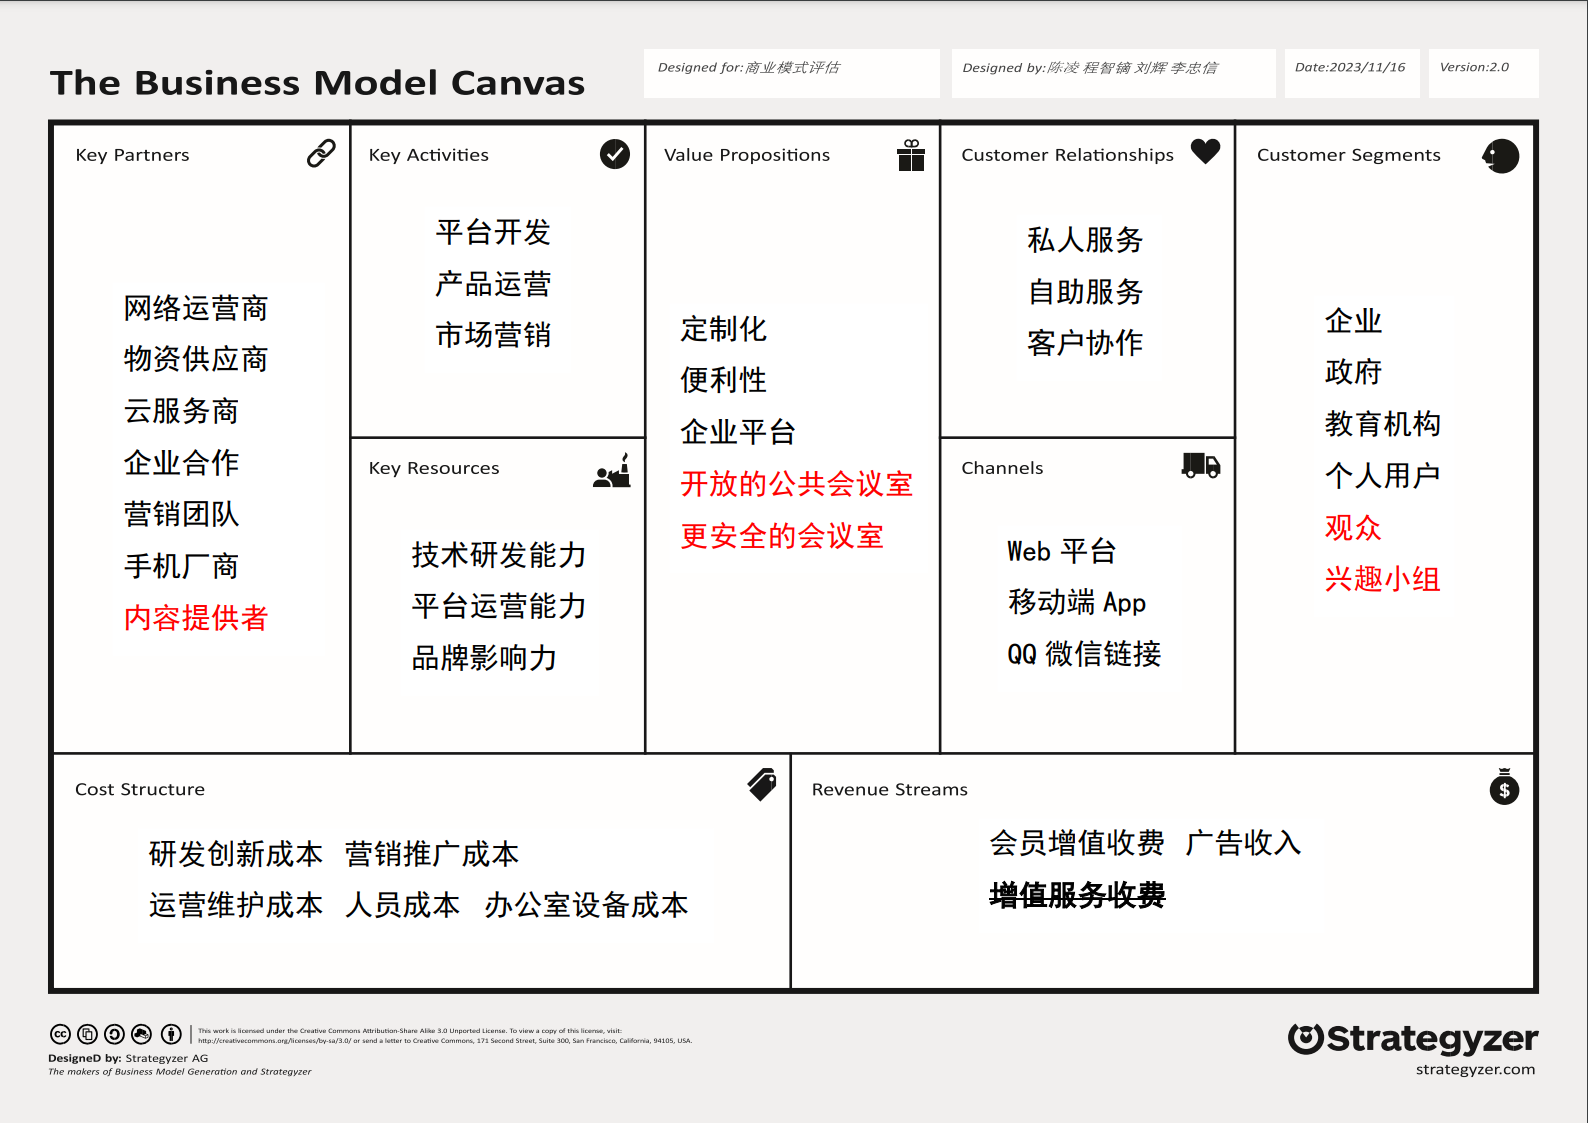
\includegraphics[scale=0.3]{png/更新画布}
        \caption{}
    \end{figure}

    \subsection{新画布优点}


    1.
    在免费增值商业模式中融入了多边平台商业模式


    2.
    提供了更优质的价值主张,包括开放的会议室、更高的安全性控制、通讯录功能等, 提高用户的使用体验,吸引更多种类的用户,
    使得更多的用户愿意为增值服务买单


    3.
    开放的会议室能同时吸引内容创作者,如公开课讲师、兴趣小组创作者,同时吸引更多的用户。这同时也为广告营收夯实基础。


    4.
    虽然研发成本会随着提供更优质的价值主张而小幅增大,但是运营维护成本会随着一些不必要的免费权益的缩减而减小



    
\end{document}
